\chapter{Aplicacion}

\section{Introducción}
La siguiente figura ofrece una visión general de los conceptos de capa de aplicación y sus relaciones, esta capa soporta los componentes de la empresa con servicios de aplicación. Muchos de los conceptos se han inspirado en el estándar UML 2.0 [7], [10], ya que este es el lenguaje dominante y el estándar que se usa hoy en día describir las aplicaciones de software. 

\begin{figure}[th!]
	\centering
	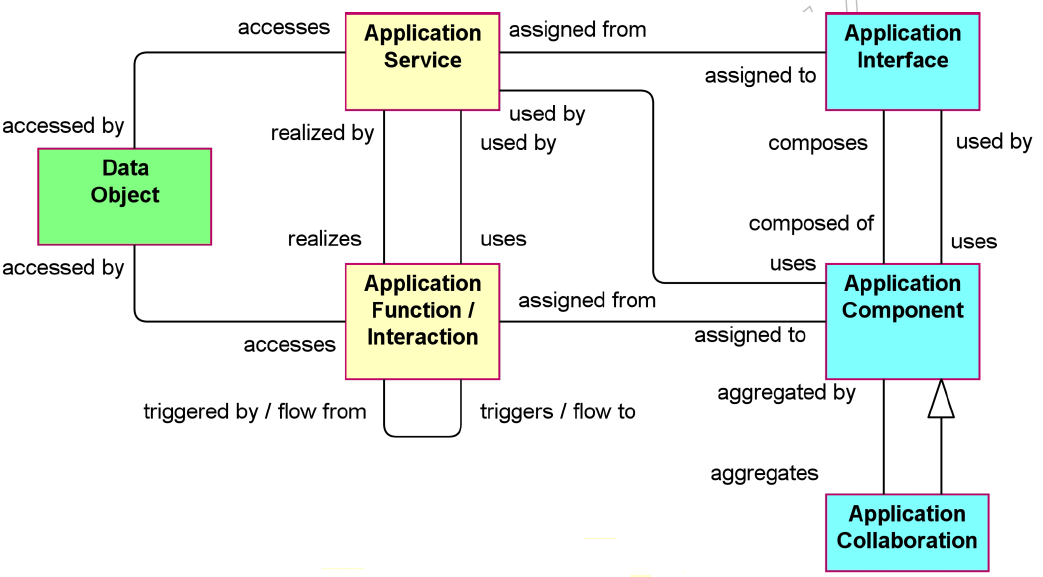
\includegraphics[width=0.7\linewidth]{arquitectura/imagenes/aplicacion}
	\caption{Capa de Aplicación}
	\label{aplicacion}
\end{figure}

Esta figura no muestra todas las relaciones permitidas: cada concepto en el lenguaje puede tener relaciones de composición, agregación y especialización con conceptos del mismo tipo; Además, existen relaciones indirectas que pueden derivarse.
\newpage

\section{Punto de Vista de Comportamiento de Aplicación}

\subsection{Modelo}

\begin{figure}[th!]
	\centering
	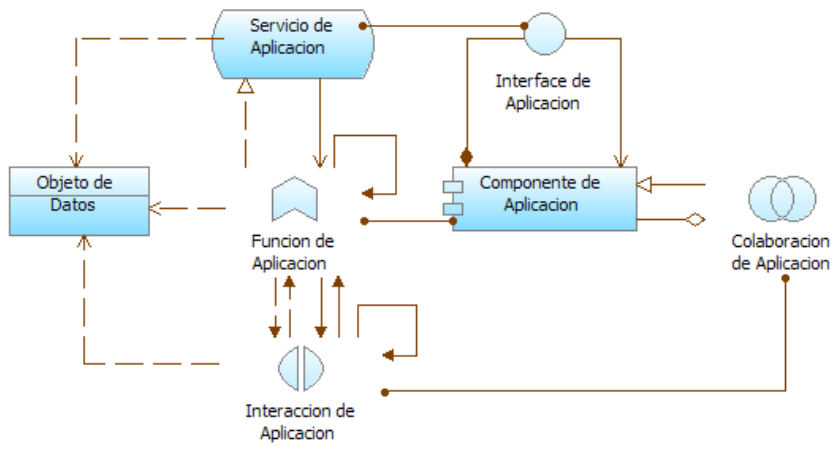
\includegraphics[width=0.5\linewidth]{arquitectura/imagenes/modeloComportamientoAplicacion}
	\caption{Metamodelo de Punto de Vista de Comportamiento de Aplicación \cite{pun7}}
	\label{fig:metamodelo de punto de vista de comportamiento de aplicación}
\end{figure}
El punto de vista del comportamiento de la aplicación describe el comportamiento interno de una aplicación, por ejemplo, cuando realiza uno o más servicios de aplicación. Este punto de vista es útil para diseñar el comportamiento principal de las aplicaciones, o para identificar la superposición funcional entre diferentes aplicaciones.

\subsection{Caso de estudio}
\begin{figure}[th!]
	\centering
	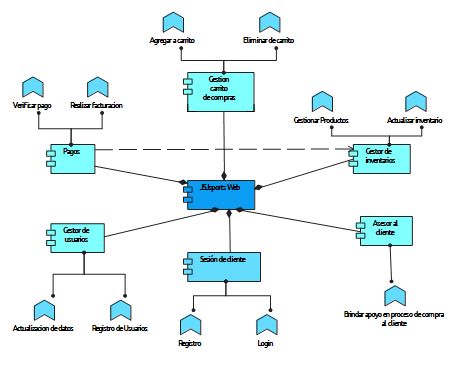
\includegraphics[width=0.6\linewidth]{arquitectura/imagenes/VistaComportamientoAplicacion}
	\caption{Punto de Vista Comportamiento de Aplicación}
	\label{fig:vistacomportamientoaplicacion}
\end{figure}
En la figura 6.3 se observa el componente principal de la empresa JSJSports, que esta conformada por varios componentes los que a su vez tienen diferentes funciones.
\newline
El componente pagos tiene dos funciones principales las cuales son verificar el pago y	realizar la facturación, este componente a su vez llama al componente de gestor de inventario que se encarga de gestionar los productos y actualizar el inventario de los mismos, el componente gestor de carrito de compras se encarga de agregar y eliminar los diferentes productos seleccionados por el cliente del carrito.
El componente de gestor de usuario se encarga de actualizar los datos y el registro de usuarios, el componente de sesión de cliente, se encarga del registro y el login que realiza el cliente para ingresar al sistema y finalmente el componente asesor de cliente que se encarga de establecer comunicación entre el asesor y el usuario para brindar apoyo en el proceso de compra.
\newpage

\section{Punto de Vista de cooperación de Aplicación}

\subsection{Modelo}

\begin{figure}[th!]
	\centering
	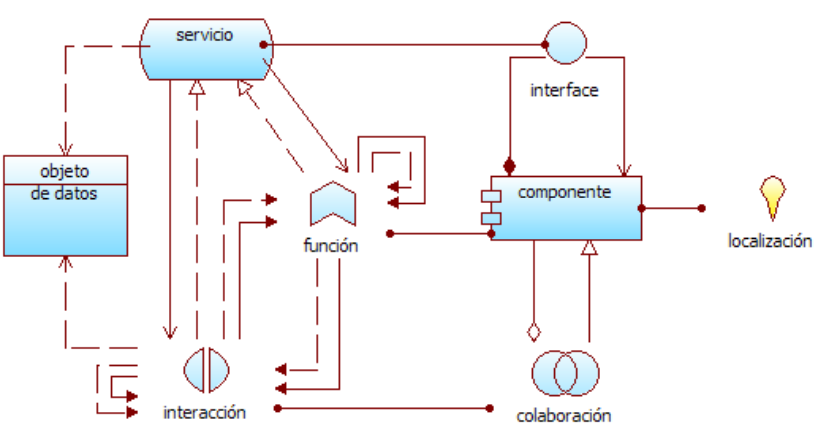
\includegraphics[width=0.5\linewidth]{arquitectura/imagenes/modeloCooperacionAplicacion}
	\caption{Metamodelo de Punto de Vista de Cooperación de Aplicación \cite{pun8}}
	\label{fig:metamodelo de punto de vista de cooperación de aplicación}
\end{figure}

El punto de vista Cooperación de Aplicación describe las relaciones entre los componentes de las aplicaciones en términos de los flujos de información entre ellos o en términos de los servicios que se ofrecen y utilizan. Este punto de vista se suele utilizar para crear una visión general del entorno de aplicación de una organización. Este punto de vista también se utiliza para expresar la cooperación (interna) o la orquestación de servicios que juntos apoyan la ejecución de un proceso de negocio.

\subsection{Caso de estudio}
\begin{figure}[th!]
	\centering
	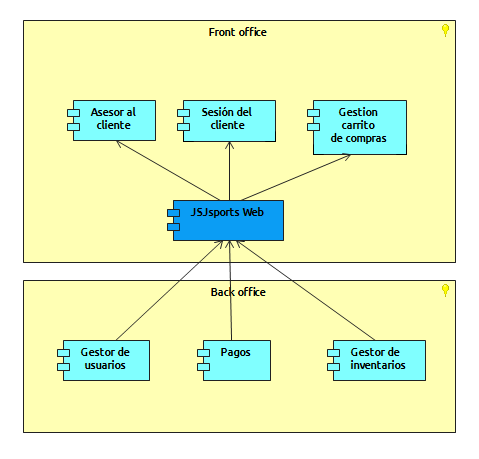
\includegraphics[width=0.5\linewidth]{arquitectura/imagenes/VistaCooperacionAplicacion}
	\caption{Punto de Vista Cooperación de Aplicación}
	\label{fig:vistacooperacionaplicacion}
\end{figure}


Como se puede ver en la figura se divide la aplicación en dos ubicaciones una que es visible y tiene acceso para el usuario, el front office y la otra que es ya la correspondiente al back end de la aplicacion que es el back office el cual no es de acceso directo para el usuario, allí se tiene la lógica de la aplicación y la persistencia de la misma.
\newline
En el back office se puede observar el gestor de pagos, el de inventarios y el de usuarios, en la parte del front office se tiene todo el componente de JSJSport web que actúa como puente entre el front office y el back office, ademas de este, tambien encontramos en el front office el componente de asesoria y el de sesión del cliente, y el componente que gestiona el carrito de compras del usuario que le permite realizar las compras.

\newpage

\section{Punto de Vista de Estructura de aplicación}

\subsection{Modelo}

\begin{figure}[th!]
	\centering
	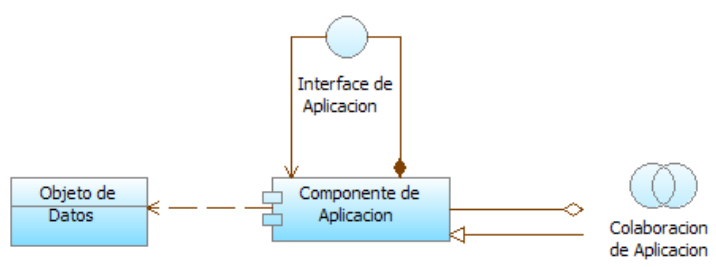
\includegraphics[width=0.7\linewidth]{arquitectura/imagenes/modeloEstructuraAplicacion}
	\caption{Metamodelo de Punto de Vista de Estructura de Aplicación \cite{pun9}}
	\label{fig:metamodelo de punto de vista de estructura de aplicación}
\end{figure}
El punto de vista de Estructura de la aplicación muestra la estructura de una o más aplicaciones o componentes. Este punto de vista es útil para diseñar o comprender la estructura principal de aplicaciones o componentes y los datos asociados, por ejemplo, para descomponer la estructura del sistema en construcción o para identificar componentes de aplicación heredados que son adecuados para la migración/integración.

\subsection{Caso de estudio}

\newpage

\section{Punto de Vista de Uso de Aplicación}

\subsection{Modelo}

\begin{figure}[th!]
	\centering
	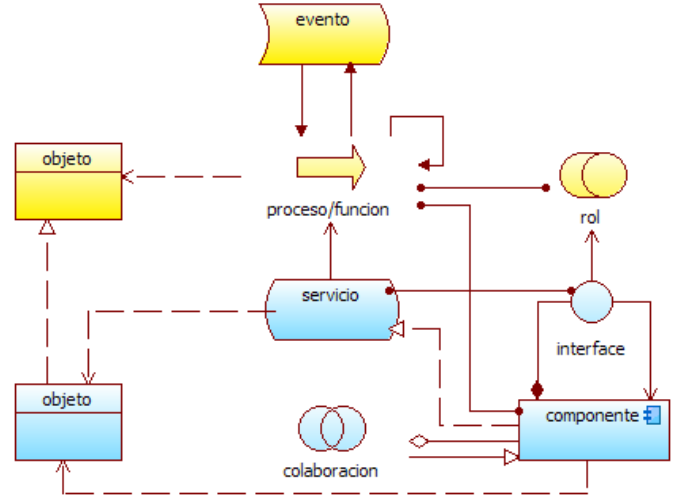
\includegraphics[width=0.5\linewidth]{arquitectura/imagenes/modeloUsoAplicacion}
	\caption{Metamodelo de Punto de Vista de Uso de Aplicación \cite{pun10}}
	\label{fig:metamodelo de punto de vista de uso de aplicación}
\end{figure}
El punto de vista Uso de aplicación describe cómo se utilizan las aplicaciones para soportar uno o más procesos empresariales y cómo se utilizan en otras aplicaciones. Se puede utilizar en el diseño de una aplicación mediante la identificación de los servicios necesarios por los procesos de negocio y otras aplicaciones, o en el diseño de procesos de negocio mediante la descripción de los servicios que están disponibles.

\subsection{Caso de estudio}

\newpage

